%! Author = lili
%! Date = 4/27/26

\section{Begrifflichkeiten}
\defin{Vererbung}
\defin{Variabilität}
\defin{Genetik}
\defin{asexFort}
\defin{sexFort}

\section{Chromosome}
\defin{Karyotyp}
\frage{menschchromosomen}

\begin{figure}[H]
    % TODO Bild 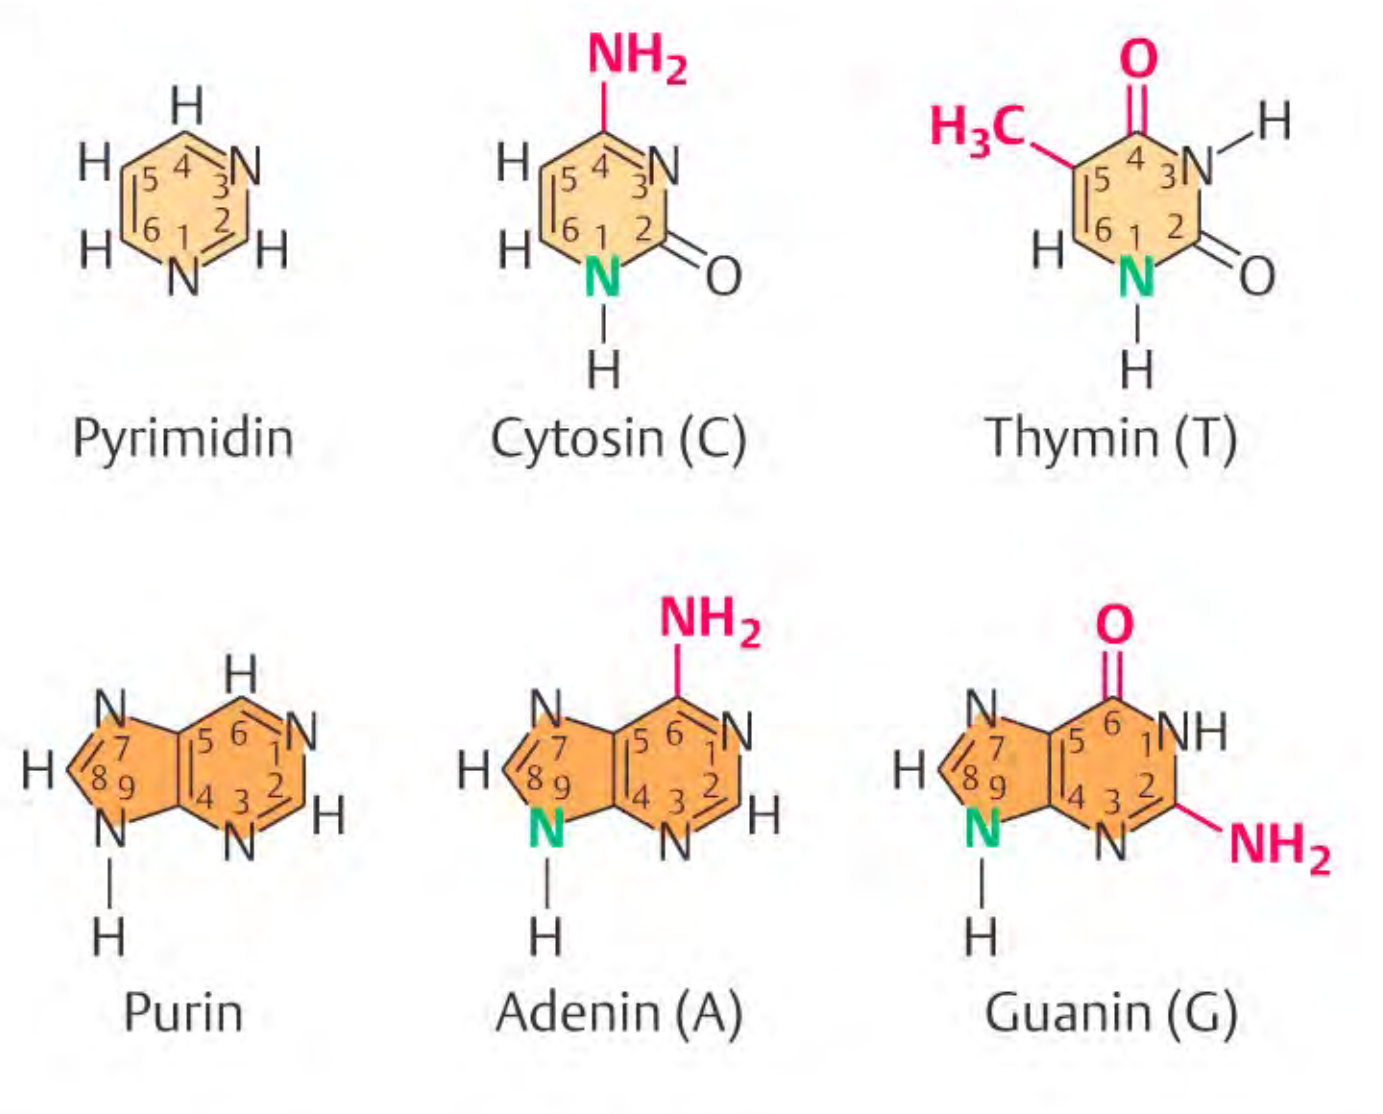
\includegraphics[width=\textwidth]{bilder/basen}
    \caption{Abbildung eines Mataphase-Chromosoms.}\label{fig:figure}
    % TODO Bildverdeckung
\end{figure}

\defin{Telomer}
\defin{Centromer}
\defin{Kinetochor}
\defin{Mikrotubuli}
\defin{Chromatid}

% TODO warum Farbkörperchen im Zellkern

\begin{figure}[H]
    % TODO Bild 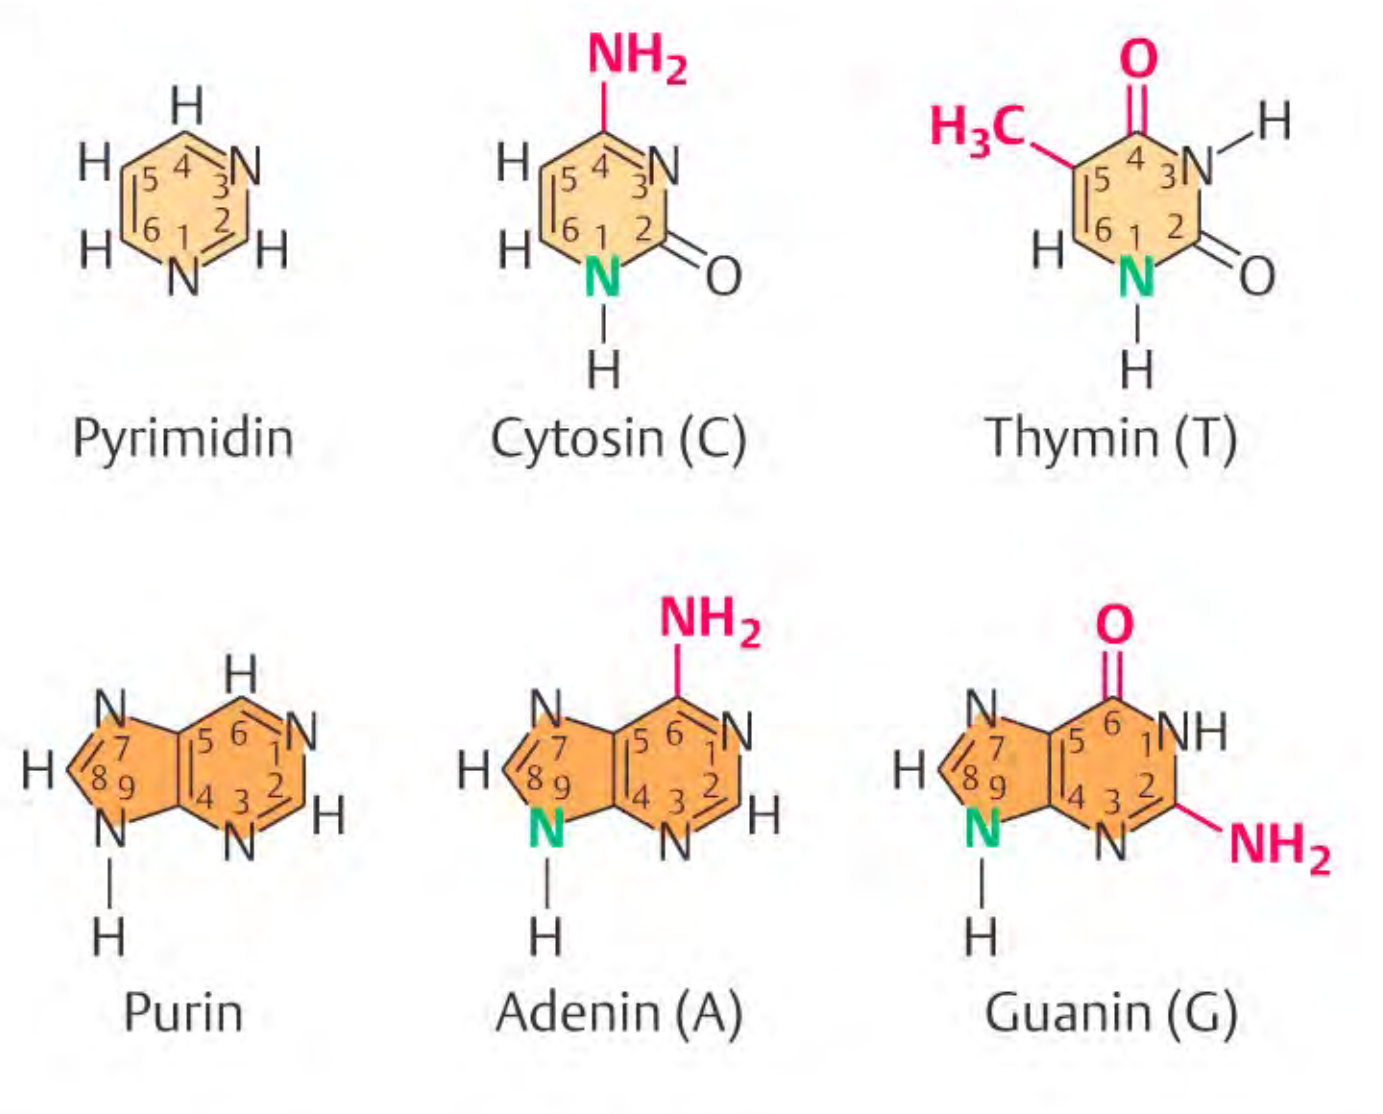
\includegraphics[width=\textwidth]{bilder/basen}
    \caption{Verschiedene Chromatin-Bereiche im Chromosom.}\label{fig:figure}
    % TODO Bildverdeckung
\end{figure}
\frage{wenigac}
\defin{Cohesin}

\section{Zellzyklus und Zellteilung}

\begin{figure}[H]
    \begin{subfigure}[t]{0.45\textwidth}
        \centering
        % TODO Bild 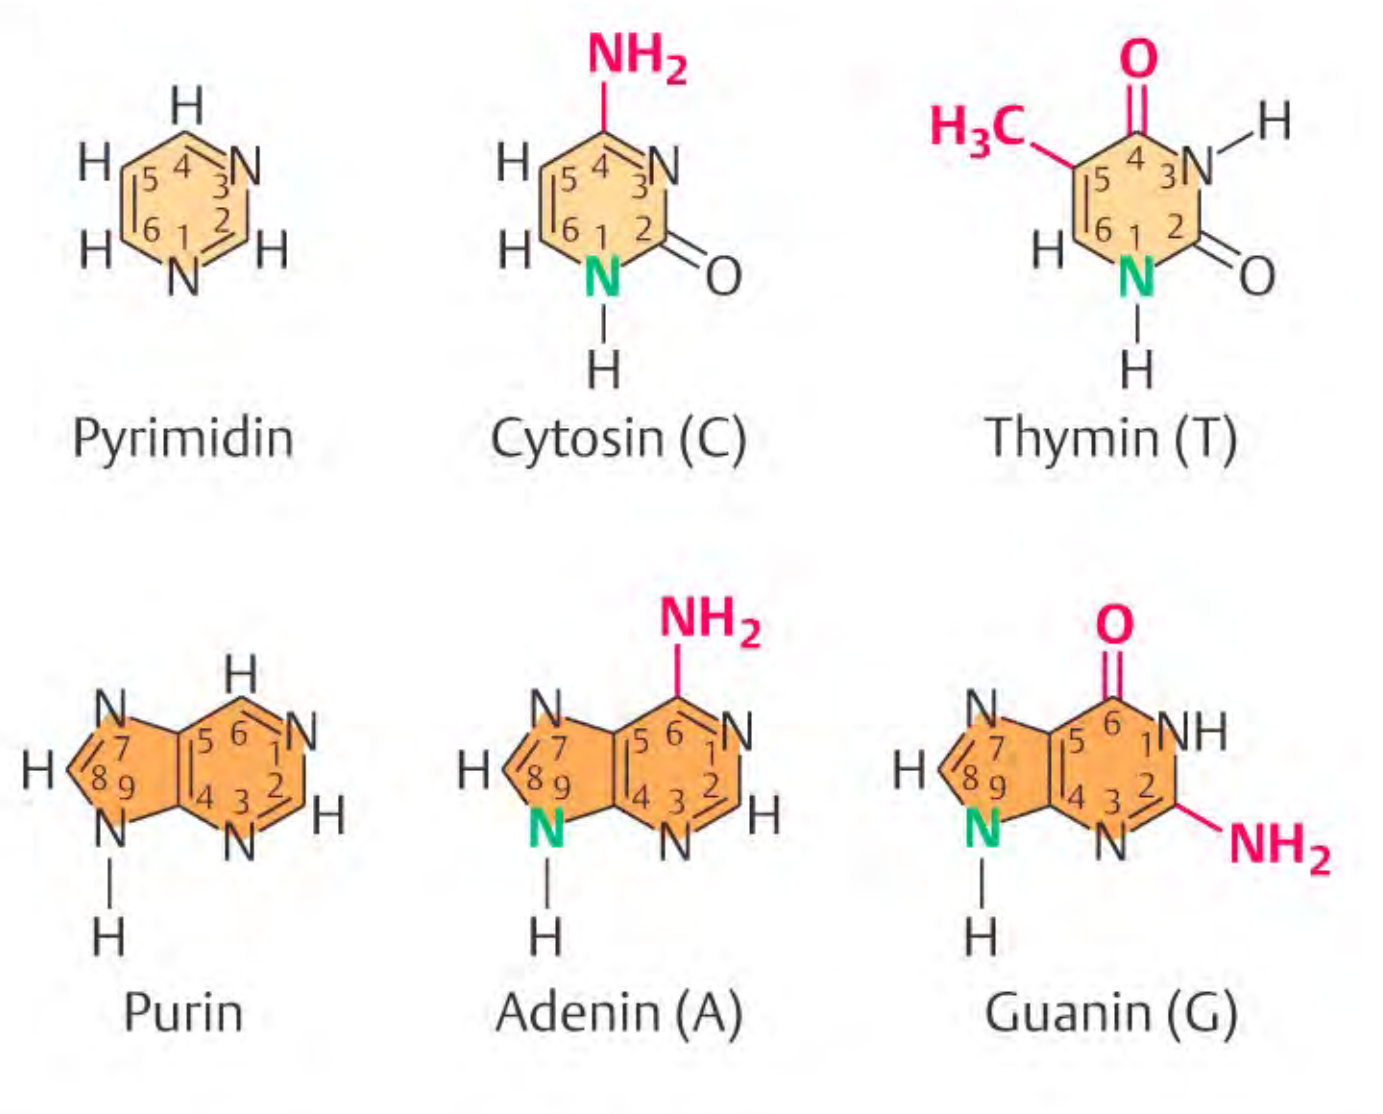
\includegraphics[width=\textwidth]{bilder/basen}
        % TODO Bildverdeckung
        \caption{Mit Fokus auf die Zellteilung.}\label{fig:figure}
    \end{subfigure}
    \hfill
    \begin{subfigure}[t]{0.45\textwidth}
        \centering
        % TODO Bild 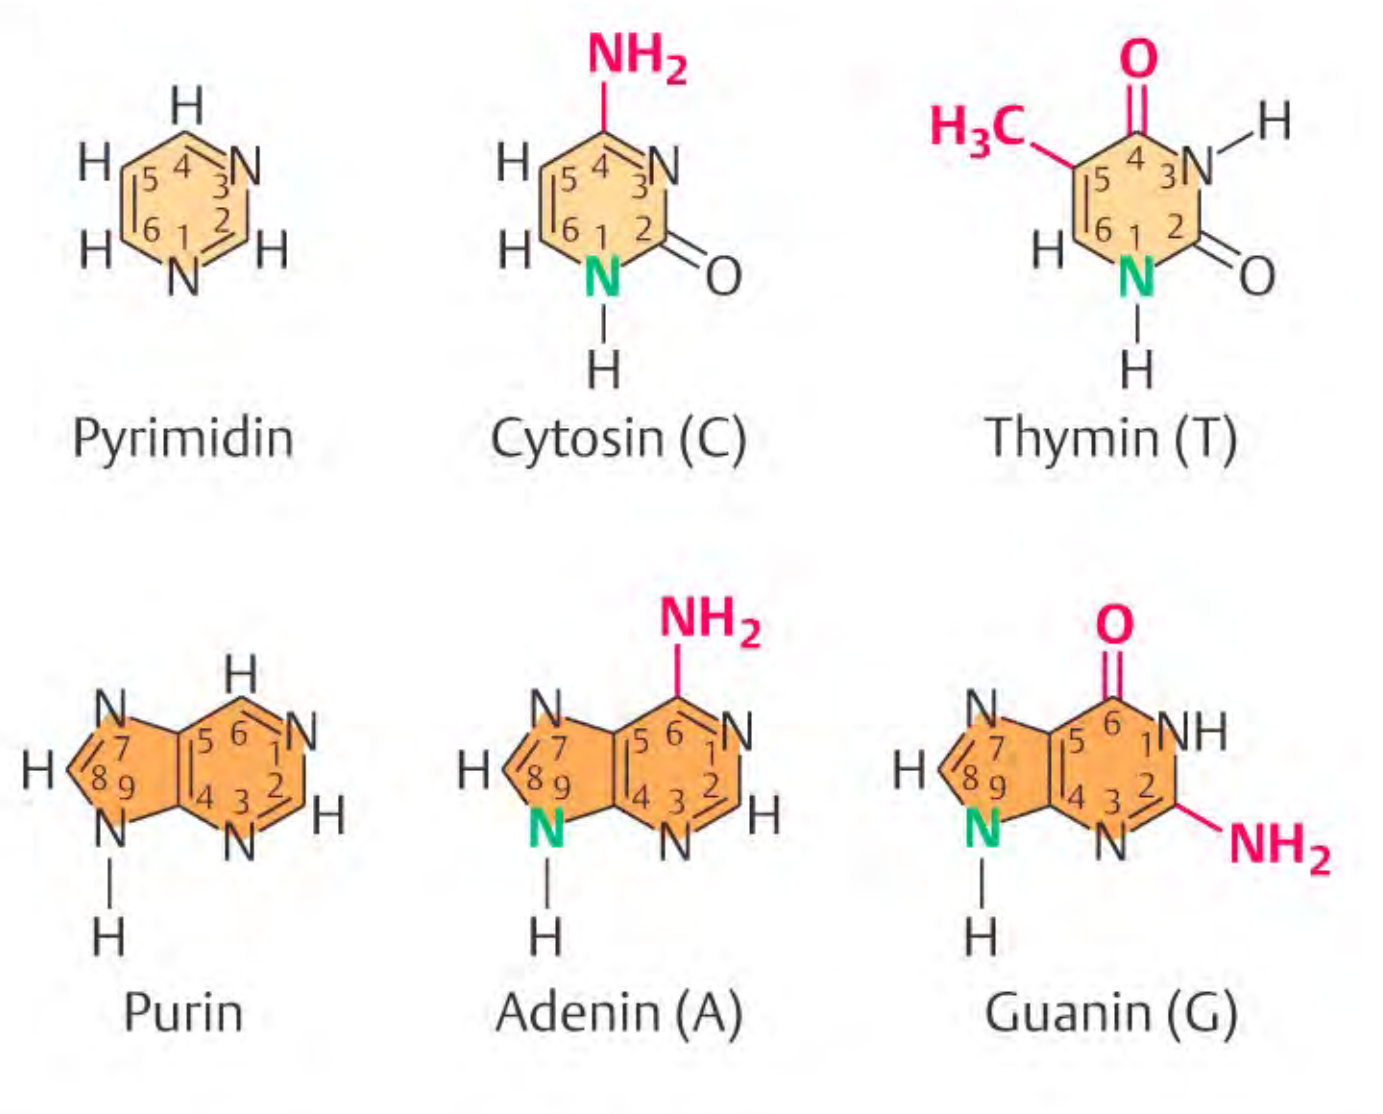
\includegraphics[width=\textwidth]{bilder/basen}
        % TODO Bildverdeckung
        \caption{Mit Fokus auf die Chromosomen.}\label{fig:figure}
    \end{subfigure}
    \caption{Verschiedene Betrachtungsweisen des Zellzyklus.}\label{fig:figure}
\end{figure}


\begin{figure}[H]
    % TODO Bild 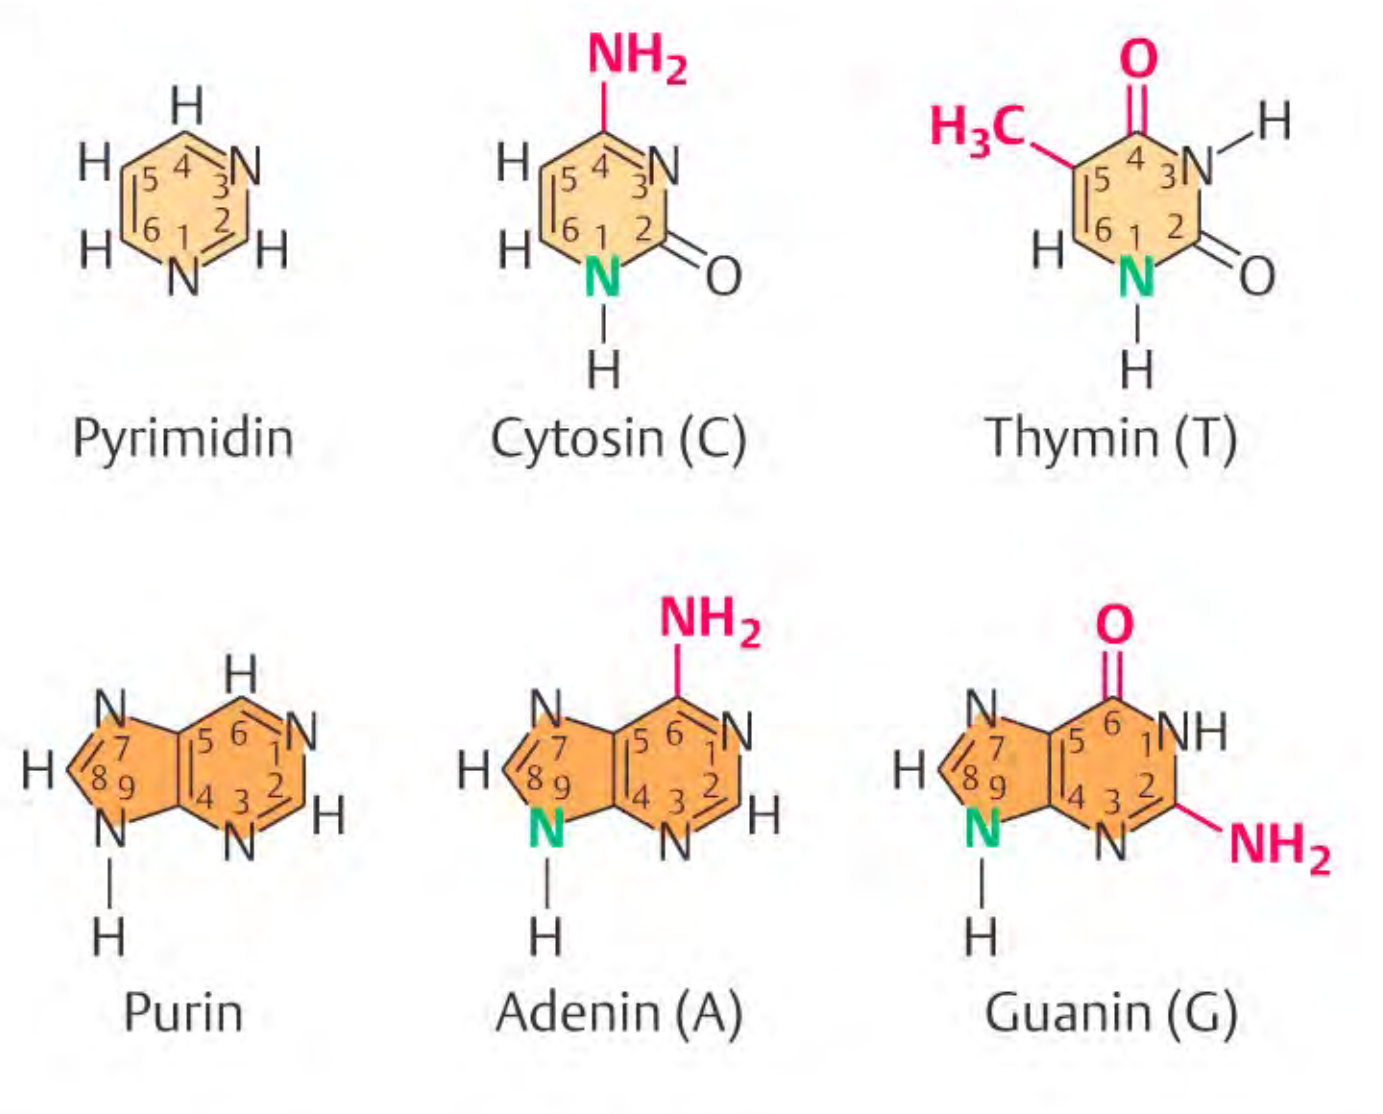
\includegraphics[width=\textwidth]{bilder/basen} F 20
    \caption{Menge an DNA, RNA und Proteinen im Verlauf des Zellzyklus.}\label{fig:figure}
\end{figure}

\frage{wannchromo}

